\section{Mechanische Grundlagen}
In den vorgestellten Konzepten werden verschiedene mechanische Bauteile verwendet. Dabei werden einfache Teile wie Rohre, Klemmen und Schl\"{a}uche als trivial angenommen und es wird nicht weiter auf die Eigenschaften dieser Teile eingegangen. Kompliziertere Bauteile sollen hier allerdings kurz erl\"{a}utert werden, um das Verst\"{a}ndnis f\"{u}r deren Funktion zu vereinfachen und die Anwendung zu verstehen.
\\\\
Da der aufgebaute Aerosolstrom durch ein System von mehreren Rohren und Schl\"{a}uchen geleitet werden muss und gegebenenfalls auch umgeleitet werden muss, wird ein Ventil ben\"{o}tigt. Ein weiteres Bauteil sind Luftfilter, um die zum Mischen verwendete Umgebungsluft zu reinigen. Letztendlich werden noch Str\"{o}mungsmaschinen f\"{u}r einige Konzepte ben\"{o}tigt, um dem Strom eine konstante Geschwindigkeit zu geben.

\subsection{Ventile}
Ein Ventil ist ein Bauteil zur Absperrung oder Regelung des Durchflusses von Fluiden. Innerhalb des Bauteils wird ein Verschlussteil nahezu parallel zur Str\"{o}mungsrichtung des Fluids bewegt. Die Str\"{o}mung kann reduziert oder unterbrochen, indem das gesamte Verschlussteil an eine passend geformte \"{O}ffnung gepresst wird. Ventile haben die Eigenschaft \"{u}ber den gesamten Stellbereich ein gleichm\"{a}{\ss}iges Str\"{o}mungsbild zu besitzen, weshalb sie sich gut f\"{u}r Regelaufgaben eignen.
\\\\
Ventile lassen sich in vier Kategorien einteilen. Durchgangsventile reduzieren Str\"{o}mungen und der Eintritt liegt in der selben Richtung wie der Austritt. Eckventile leiten den Strom um, indem Ein- und Austritt im rechten Winkel zueinander liegen, w\"{a}hrend Schr\"{a}gventile die Str\"{o}mungsrichtung um \(45^\circ\) \"{a}ndern. Die f\"{u}r diese Arbeit wichtigen Ventile sind Drei-Wege-Ventile, die f\"{u}r das kontrollierte Mischen von Fluidstr\"{o}men verwendet werden. Bei allen Kategorien kann man noch Unterschiede in den Bet\"{a}tigungsarten machen, um jedoch ein Signal f\"{u}r den Messbereich zu haben, werden hier elektronische Bet\"{a}tigungen bevorzugt\cite{ventil}.
\begin{figure}[H]
        \myfloatalign
        {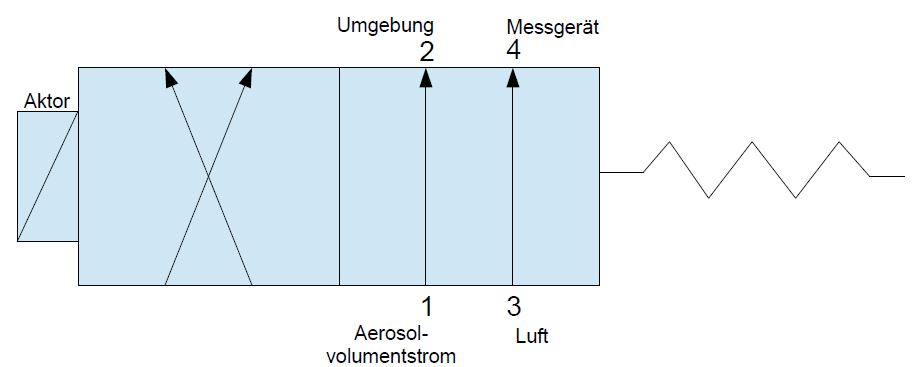
\includegraphics[width=.9\linewidth]{gfx/concepts/ventil_feder.jpg}} \quad
        \caption[Schaltm\"{o}glichkeiten von 4/2-Wegeventilen]
        {Schaltm\"{o}glichkeiten von 4/2-Wegeventilen}
        \label{fig:ventil}
\end{figure}
\newpage
\subsection{Luftfiltersysteme}
Als Luftfilter werden alle Abscheider bezeichnet, die Aerosole oder andere unerw\"{u}nschte Schwebstoffe aus der Luft herausfiltern. Es gibt viele verschiedene Bauarten von Luftfiltersystemen, doch es werden nur Trockenfilter, Zyklonabscheider und elektrostatische Luftfilter verwendet, weshalb die fl\"{u}ssigkeitsbasierten Filter hier nicht wieder erw\"{a}hnt werden. \\
Trockenfilter bestehen aus ringf\"{o}rmig oder rechteckig angeordneten Gebilde, die zickzackf\"{o}rmiges Gewebe als Filterelement haben. Die Faltung vergr\"{o}{\ss}ert die Filterfl\"{a}che und verringert den Str\"{o}mungswiderstand. Die kontaminierte und ungefilterte Luft wird ausserhalb des Zylinders angesaugt und die gefilterte saubere Luft wird innerhalb der Lamellen weitergeleitet. Die Partikel und Schwebeteilchen bleiben in den Gewebefalten h\"{a}ngen.\\
Elektrofilter finden haupts\"{a}chlich Anwendung bei der Abscheidung von Aerosolen. Im Filter werden die Staub- oder Aerosolpartikel elektrostatisch aufgeladen und an den Elektrodenfl\"{a}chen abgeschieden. In getakteten Abfolgen werden die aufgefangenen Verschmutzungen maschinell entfernt und in einem Trichter gesammelt. Der Vorteil dieser Filter im Vergleich zu den Trockenfiltern ist, dass es keine Filtereins\"{a}tze gibt, die ausgetauscht werden m\"{u}ssen, allerdings sind die elektrostatischen Filter wesentlich teurer als die Einwegfilter mit Gewebeeinsatz.\\
Zyklonabscheider werden dazu genutzt, um Partikel einer bestimmten Gr\"{o}{\ss}e aus dem Strom herauszufiltern. Diese finden ihre Anwendung, um nur Partikelgr\"{o}{\ss}en durchzulassen, die f\"{u}r die verwendeten Messger\"{a}te erkennbar sind. Sie sind allerdings zu ineffizient, um die Luft von allen Partikeln zu reinigen, weshalb sie nur zur Aufbereitung des Partikelstroms in Frage kommen\cite{filter}.

\subsection{Str\"{o}mungsmaschinen}
Da es eines der Ziele ist, einen konstanen Partikelstrom durch den Versuchsaufbau zu leiten, wird eine Str\"{o}mungsmaschine ben\"{o}tigt, um den Strom in Bewegung zu bringen. Daf\"{u}r gibt es verschiedene M\"{o}glichkeiten. F\"{u}r fl\"{u}ssige und feste Stoffe werden Pumpen verwendet, die bei der Str\"{o}mungserzeugung eine Druckerh\"{o}hung mit sich bringen. Auch wenn in vielen Messger\"{a}ten laut Datenblatt die Luft mit Pumpen angezogen wird, werden dort keine Pumpen verwendet, sondern sogenannte Verdichter. Verdichter saugen durch ein Vakuum Gase an und erzeugen so Str\"{o}mungen. Allerdings ist auch hier eine Druckerh\"{o}hung unvermeidbar. Um keine hohen Dr\"{u}cke in den Leitungen zu haben, werden Gebl\"{a}se, oder Ventilatoren verwendet. Die Ventilatoren erzeugen durch ein angetriebenes Laufrad einen Luftstrom und erzeugen so eine Str\"{o}mung in die man nun das Gas einflie{\ss}en lassen kann\cite{maschine}.